\problemname{Sortera spellistan}

Du har en spellista med $N$ låtar med olika längder, som ligger i en given ordning. Du vill sortera listan så att de kortaste
låtarna kommer först och de längsta låtarna kommer sist.

Vad är det minsta antalet platsbyten du behöver göra för att få listan sorterad?
Vid ett platsbyte väljer du två intilliggande låtar och byter plats på
dem.

\begin{figure}[ht!]
\centering
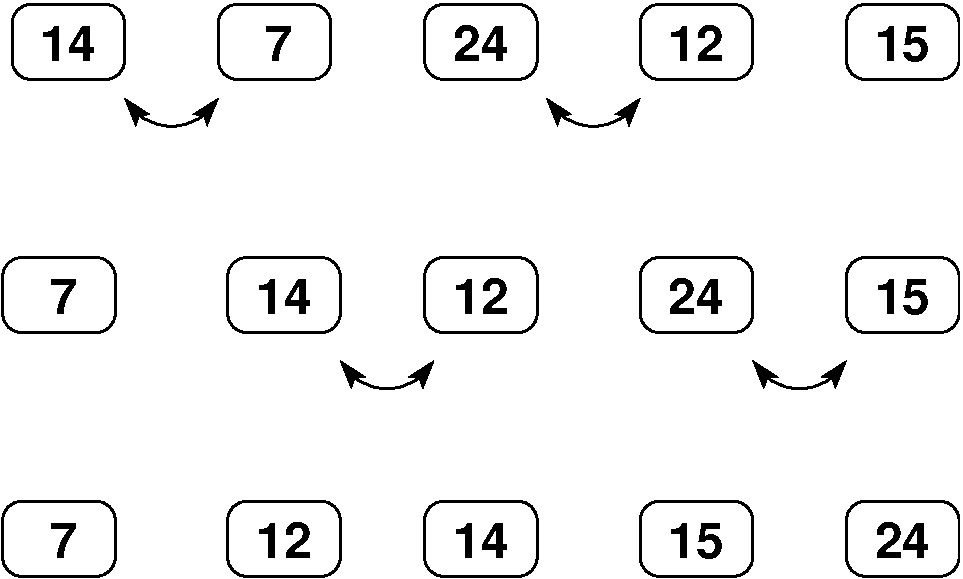
\includegraphics[width=5cm]{sorterafig.pdf}
\caption{Översta raden visar låtarnas startordning i första exemplet. Pilarna visar platsbytena som behöver göras för att göra spellistan sorterad (understa raden)}
\end{figure}

\section*{Indata}

På första raden av indatan står ett heltal $N$, där $1\le N \le
1000$, antalet låtar. Därefter följer $N$ rader vardera innehållande ett heltal mellan 1 och 1000,
längden på varje låt i den ordning de ligger från början. Alla låtarna
har olika längd.

\section*{Utdata}

Programmet ska skriva en rad med ett heltal, det minsta antalet
platsbyten som behöver göras för att sortera spellistan.

\section*{Delpoäng}

För att få 60 poäng räcker det att programmet klarar fall med $N\le 100$.
